%----------------------------------------------------------------------------------------
%    PAGE ADJUSTMENTS
%----------------------------------------------------------------------------------------

\documentclass[12pt,a4paper,hidelinks]{article}            % Article 12pt font for a4 paper while hiding links
\usepackage[margin=1in]{geometry}                          % Required to adjust margins

%----------------------------------------------------------------------------------------
%    TYPE SETTING PACKAGES
%----------------------------------------------------------------------------------------

\usepackage[utf8]{inputenc}                                % Accept different input encodings
\usepackage[russian]{babel}                                % Russian language/hyphenation 
\usepackage{amsmath,amsfonts,amsthm,amssymb,thmtools}      % Math packages to use equations
\usepackage[retainorgcmds]{IEEEtrantools}
\usepackage{siunitx}                                       % Scientific units and numbering
\usepackage[usenames,dvipsnames,svgnames,table]{xcolor}    % Set color of text/background
\linespread{1.2}                                           % Default line spacing size
\usepackage{microtype}                                     % Improves spacing in the document
\usepackage{setspace}                                      % Set line spacing dynamically
\usepackage{tocloft}                                       % List adjustments including ToC

%----------------------------------------------------------------------------------------
%    FIGURES
%----------------------------------------------------------------------------------------

\usepackage{graphicx}                                      % Required for the inclusion of images
\usepackage{tikz}
\graphicspath{{images/}}                               % Specifies picture directory
\usepackage{float}                                         % Allows putting an [H] in \begin{figure}
\usepackage{wrapfig}                                       % Allows in-line images

\usepackage{hyperref}                                      % References
\usepackage{cleveref}                                      % Better References
%\crefname{lstlisting}{listing}{listings}
%\Crefname{lstlisting}{Listing}{Listings}
\crefname{figure}{figure}{figures}
\Crefname{figure}{Figure}{Figures}

%----------------------------------------------------------------------------------------
%    INCLUDE CODE
%----------------------------------------------------------------------------------------

\usepackage{listings}                                      % Package so code looks pretty
\lstset{
language=C,                                                % Choose the language
basicstyle=\footnotesize,                                  % The size of the fonts used
numbers=left,                                              % Where to put the line-numbers
numberstyle=\footnotesize,                                 % The size of the line-numbers
stepnumber=1,                                              % The step line-numbers
numbersep=5pt,                                             % How far the line-numbers are from the code
backgroundcolor=\color{white},                             % Choose the background color
showspaces=false,                                          % Show spaces adding partiular underscores
showstringspaces=false,                                    % Underline spaces within strings
showtabs=false,                                            % Show tabs within strings adding particular underscores
frame=single,                                              % Adds a frame around the code
tabsize=2,                                                 % Sets default tabsize to 2 spaces
captionpos=b,                                              % Sets the caption-position to bottom
breaklines=true,                                           % Sets automatic line breaking
breakatwhitespace=false,                                   % Sets if automatic breaks should only happen at whitespace
escapeinside={\%*}{*)}                                     % If you want to add a comment within your code
}

%----------------------------------------------------------------------------------------
%    EXTRAS
%----------------------------------------------------------------------------------------

\usepackage{attachfile}                                    % Attach files to your document
\usepackage{fancyhdr}                                      % Fancy Header

%----------------------------------------------------------------------------------------
%    Extra commands
%----------------------------------------------------------------------------------------

% Concise referencing
\newcommand{\eqnref}[1]{\eqref{#1}}
\newcommand{\secref}[1]{Section \ref{#1}}
\newcommand{\figref}[1]{Figure \ref{#1}}
\newcommand{\lemref}[1]{Lemma \ref{#1}}
\newcommand{\corref}[1]{Corollary \ref{#1}}
\newcommand{\thmref}[1]{Theorem \ref{#1}}
% Real numbers
\newcommand{\Real}[1]{\mathbb{R}^{#1}}
% Complex numbers
\newcommand{\Complex}[1]{\mathbb{C}^{#1}}
% Integers
\newcommand{\Integer}[1]{\mathbb{Z}^{#1}}
% Rank operator
\DeclareMathOperator{\rank}{\textnormal{rank}}
% Vec operator
\newcommand{\vecop}{\textnormal{vec}}
% Norm
\newcommand{\norm}[1]{\left|\left|#1\right|\right|}
% Trace
\newcommand{\trace}{\textnormal{tr}}
% Range
\newcommand{\range}{\textnormal{range}}
% Partial derivative
\newcommand{\pd}[2]{\dfrac{\partial #1}{\partial #2}}
% Complete derivative
\newcommand{\dd}[2]{\dfrac{d #1}{d #2}}
% Complete derivative, second order
\newcommand{\dds}[2]{\dfrac{d^2 #1}{d {#2}^2}}
% Limit to N / N
\newcommand{\limover}[1]{\lim_{#1 \rightarrow \infty} \dfrac{1}{#1}}
% Display style sum
\newcommand{\dsum}{\displaystyle\sum}
% arg min and arg max
\newcommand{\argmax}[1]{\underset{#1}{\operatorname{arg~max}}}
\newcommand{\argmin}[1]{\underset{#1}{\operatorname{arg~min}}}
%---------------------------------------------------------------------------
% Create theorem without number
\declaretheoremstyle[headfont=\bfseries,notefont=\bfseries,bodyfont=\itshape,notebraces={}{},headpunct={},postheadspace=1em]{mystyle}
\declaretheorem[style=mystyle,numbered=no,name=Теорема]{thm-hand}

\newtheorem{theorem}{Теорема}
\newtheorem{corollary}{Следствие}[theorem]
\newtheorem{lemma}{Лемма}
\newtheorem{exmp}{Пример}
\newtheorem*{remark}{Замечание}
\newtheorem*{mdef}{Определение}
\newtheorem*{mex}{Пример}


\begin{document}

%----------------------------------------------------------------------------------------
%    COMMANDS
%----------------------------------------------------------------------------------------

\setlength\parindent{0pt}                                  % Removes all indentation from paragraphs
\renewcommand*\thesection{\arabic{section}}                % Renew section numbers
\renewcommand{\labelenumi}{\alph{enumi}.}                  % Section ordered numbering
\let\oldvec\vec                                            % Save the old vector style
\renewcommand{\vec}[1]{\oldvec{\mathbf{#1}}}               % Set vectors to look like vectors

\renewcommand{\contentsname}{Table of Contents}            % Make ToC actually say ToC
\addtocontents{toc}{~\hfill\textbf{Page}\par}              % Add 'page' to top of ToC
\renewcommand{\cftsecleader}{\cftdotfill{\cftdotsep}}      % Makes dots leading up to page number
\setcounter{tocdepth}{3}                                   % Depth of ToC
\setcounter{lofdepth}{3}                                   % Depth of LoF

\pagestyle{fancy}                                          % Fancy page style for headers
\setlength{\headheight}{15pt}                              % Change header hieght
\fancyhead[L,LO]{\fontsize{8}{10} \selectfont \firstmark}  % Adds header to left with section name
\fancyhead[R,RO]{\fontsize{8}{10} \selectfont Right}       % Adds header to right
\definecolor{grey}{HTML}{cccccc}                           % The next 4 lines modifies the header (color)
\renewcommand{\headrulewidth}{1px}
\renewcommand{\headrule}{{\color{grey}%
\hrule width\headwidth height\headrulewidth%
\vskip-\headrulewidth}}

\numberwithin{equation}{section}                           % Number equations within sections
\numberwithin{figure}{section}                             % Number figures within sections
\numberwithin{table}{section}                              % Number tables within sections
\numberwithin{lstlisting}{section}                         % Number listings within sections

% \renewcommand{\sfdefault}{phv}                             % Change default font
% \renewcommand{\familydefault}{\sfdefault}                  % Use default font everywhere


%----------------------------------------------------------------------------------------
%    TITLE PAGE
%----------------------------------------------------------------------------------------

\begin{titlepage}

\title{My Latex Header}
\author{danmir}

\vspace*{\fill}                                            % Center title page vertically

\newcommand{\HRule}{\rule{\linewidth}{0.3mm}}              % Defines horizontal lines

\center                                                    % Center everything on the page

\textsc{\Large УрФУ Мат-Мех}\\[1.5cm]
\textsc{\Large Дифференциальные уравнения}\\[0.5cm]
\textsc{\large Курс 2015 года 4 семестр (КБ-КН)}\\[0.5cm]

\HRule \\[0.4cm]
{ \huge \bfseries Лекция 1 \\ Базовые определения}\\[0.4cm]
\HRule \\[1.5cm]

\begin{minipage}{0.4\textwidth}
\begin{flushleft} \large
\emph{Авторы конспекта:}\\
\begin{tabular}{ l c r }
  Данил \textsc{Миронов (КБ-201)}\\
\end{tabular}
\end{flushleft}
\end{minipage}
~
\begin{minipage}{0.4\textwidth}
\begin{flushright} \large
\emph{Курс читает:} \\
Ряшко Л.Б. \textsc{}                                             % Professor's Name
\end{flushright}
\end{minipage}\\[4cm]

{\large \today}\\[3cm]                                              % Date, change the \today to be precise

%\includegraphics{Logo}\\[1cm]                             % Include a department/university logo

\vspace*{\fill}                                                           % Fill the rest of the page with whitespace

\end{titlepage}

\phantomsection

\newpage
\begin{mdef}
    ДУ - уравнение, связывающее $F(t,x,x',\ldots,x^{n})=0$ уравнение n-ого порядка, где $F$ - функция $t$ - независимая переменная \\
    Решение - функция $x=\psi(t)$ на $(\alpha,\beta)$ такая, что при подстановке в исходное уравнение - оно превращается в тождество по $t$ на интервале
\end{mdef}

\section{Дифференциальные уравнения первого порядка разрешенные относительно производных}
\begin{equation}\tag{1}\label{eq:1}
    \dd{x}{t}=f(t,x) \mbox{ само уравнение $F(t,x,x'')$}
\end{equation}
Еще более узко $\dd{x}{t}=f(t)$ \# Найти $x\Longrightarrow x(t)=\int f(t)dt=\underbrace{\int^{t}_{t_{0}}f(\tau)d\tau}_{\psi(t)}+C$ - общее решение
\begin{center}
	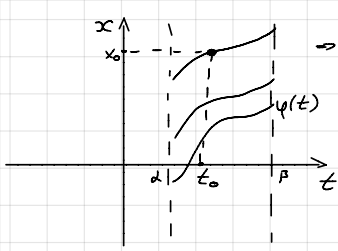
\includegraphics[scale=0.7]{images/graph1}
\end{center}
\begin{equation}\tag{2}
  x(t_0)=x_0
\end{equation}
Это доп условие приводит к задаче, имеющей единственное решение
\begin{mdef}[Задача Коши]
	Нужно добавить начальное условие
	$$ 
	   \left\{
	   \begin{aligned}
	   &\mbox{(1) } \dd{x}{t}=f(t,x)&\mbox{ - д.у}\\
	   &\mbox{(2) } x(t_0)=x_0&\mbox{ - начальное условие}\\
	   \end{aligned}
	   \right. 
	$$
\end{mdef}
При каких-то условиях задача имеет единственное решение

\section{Геометрический смысл д.у. и задачи Коши}
\begin{center}
	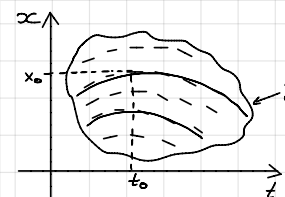
\includegraphics[scale=0.8]{images/graph2}
\end{center}
$D$ - область определения $f(t,x)$ \\
Правая часть уравнения (\ref{eq:1}) - функция $f(t,x)$ позволяет в каждой точке $D$ найти поле направлений \\
Нужно двигаться так, чтобы рис. траект. в каждой точке имела направление соответствующее полю напр. То есть двигаться вдоль поля \\
Имеем первый способ решения д.у.: по правой части строим рисунок поля, затем по полю строим решения

\newpage
\section{Аналитические методы решения ДУ}
\subsection{Уравнения с разделяющимеся переменными}
$$\dd{x}{t}=f(t)g(x)$$
{\bfseries a)} $g(x)=0$ $x_k,k=1,2,\ldots$ \\
$x\equiv x_k$ - решение (1) константы - решения \\
{\bfseries б)} $g(x)\not=0$  $\int\frac{dx}{g(x)}=\int f(t)dt$ \\
Пусть $G(x)$ - первообразная для $\frac{1}{g(x)}$ , $F(t)$ - первообразная для $f(t)$ \\
Тогда уравнение записывается $G(x)=F(t)+C$ - общее решение \\
Дальше уже другие проблемы $x=\psi(t,c)$ \\
%\begin{mex}
%    $\dd{x}{t}=\dfrac{t+1}{x}, x\not=0$ \\\\
%    $\int xdx=\int(t+1)dt$ \\\\
%    $\dfrac{x^2}{2}=\dfrac{t^2}{2}+t+C$ \\\\
%    $x^2=t^2+2t+C$
%\end{mex}
\begin{mex}
\begin{gather*}
	\dd{x}{t}=\dfrac{t+1}{x}, x\not=0 \\
	\int xdx=\int(t+1)dt \\
	\dfrac{x^2}{2}=\dfrac{t^2}{2}+t+C \\
	x^2=t^2+2t+C
\end{gather*}
\end{mex}

\subsection{Линейные уравнения}
\begin{equation}\tag{1}
  \dd{x}{t}=a(t)x+b(t)
\end{equation}
$$x_\textup{он}=x_\textup{оо}+\overline{x_\textup{чн}}$$ \\
Решение линейного неоднородного складывается из общего решения однородного и частного неоднородного $x=0$ - решение \\
\begin{equation}\tag{2}
  \dd{x}{t}=a(t)x \mbox{ - соответствующее однородное уравнение}
\end{equation}
\begin{gather*}
	\int\dfrac{dx}{x}=\underbrace{\int a(t)dt}_{A(t)} \\
	\ln|x|=A(t)+\ln C, C>0 \\ \mbox{если $C>0$ то $\ln C$ пробегает все числа} \\
	\ln|x|=\ln e^{A(t)}+\ln C \\
	|x|=\ln Ce^{A(t)} \\
	|x|=Ce^{A(t)}
\end{gather*}
Общее решение однородного уравнения \\
$$ \left[
\begin{aligned}
x&=\pm ce^{A(t)} \\
x&\equiv0 \\
\end{aligned}
\right. $$
\begin{center}
	\boxed{$$x_\textup{оо}=c_{1}e^{A(t)}$$}
	$c_1\in\Real{}$
\end{center}

\subsubsection{Метод вариации прозвольной постоянной}
\begin{gather*}
	x_\textup{оо}=ce^{A(t)}\mbox{ где $c\in\Real{}$} \\
	\overline{x}=c(t)e^{A(t)}\mbox{ - частное решение н.у (1)}\\
	\dd{\overline{x}}{t}=c'(t)e^{A(t)}+c(t)e^{A(t)}\underbrace{A'(t)}_{=a(t)}=a(t)c(t)e^{A(t)}+b(t)
	c'(t)e^{A(t)}=b(t) \\
	\dd{c}{t}=b(t)e^{-A(t)}\Rightarrow c(t)=\int b(t)e^{-A(t)}dt
\end{gather*}
Подставим в $\overline{x}$ и получим частное решение неоднородного уравнения
\begin{mex}
	$\dd{x}{t}=2\dfrac{x}{t}+t^3$ \\
	Решаем однородное $\dd{x}{t}=2\dfrac{x}{t}$ \\\\
	$\dfrac{dx}{2x}=\dfrac{dt}{t}$; $\int\dfrac{dx}{x}=2\int\dfrac{dt}{t} \Rightarrow \ln|x|=2\ln|t|+C$; $x=t^2C$ \\\\
	Метод вариации произвольной постоянной \\
	$\overline{x_\textup{чн}}=t^2C(t)$ \\
	$\overline{x_\textup{чн}}'=2tC(t)+t^2C'(t)$ \\
	Подставим в исходное уравнение: $2tC(t)+t^2C'(t)=\dfrac{2t^2C(t)}{t}+t^3$ \\
	$t^2C'(t)=t^3\Rightarrow C'(t)=t \Rightarrow C(t)=\dfrac{t^2}{2}$ \\
	Подставим обратно $\overline{x_\textup{чн}}=\dfrac{t^4}{2}$ \\
	Получим $x_\textup{он}=x_\textup{оо}+\overline{x_\textup{чн}}$ \\
	$x_\textup{он}=t^2C+\dfrac{t^4}{2}$
\end{mex}



%\begin{theorem}[Названа в честь \ldots]
%Тут условие теоремы
%\end{theorem}
%\begin{proof}
%Тут доказательство теоремы
%\end{proof}
%
%\begin{corollary}
%\end{corollary}
%
%\begin{lemma}
%\end{lemma}
%
%\begin{thm-hand}[1]
%Текст условия теоремы, которую мы сами пронумеровали
%\end{thm-hand}
%\begin{proof}
%Тут доказали теорему, которую сами пронумеровали
%\end{proof}
%
%
%
%Далее по тексту ссылаемся на теорему \itshape{(1)}
%
%\begin{equation}\tag{2.718}
%a+b=c
%\end{equation}
%
%$$ \left\{
%\begin{aligned}
%x^2+y^2&=7\\
%x+y & = 3.\\
%\end{aligned}
%\right. $$
%
%$$\dds{x}{y}$$


\end{document}